% Individual report source; existing report versions are unchanged.
% Compile with: pdflatex -jobname=DT081A_Lab3_Report_Yacoub_Dawli main_individual.tex
\documentclass[10pt,a4paper]{article}
\usepackage[T1]{fontenc}
\usepackage{lmodern}
\usepackage[margin=20mm]{geometry}
\usepackage{graphicx,amsmath,booktabs,caption,float,listings,titlesec,hyperref}
\hypersetup{hidelinks,pdftitle={Lab 3 Report — Image Processing},
  pdfauthor={Yacoub Dawli}}
\graphicspath{{../figures/}}
\setlength{\parindent}{0pt}
\setlength{\parskip}{2pt}
\setlength{\intextsep}{5pt}
\setlength{\textfloatsep}{5pt}
\titleformat{\section}{\large\bfseries}{\thesection}{0.6em}{}
\titleformat{\subsection}{\normalsize\bfseries}{\thesubsection}{0.6em}{}
\titlespacing*{\section}{0pt}{6pt}{3pt}
\titlespacing*{\subsection}{0pt}{5pt}{2pt}
\captionsetup{font=normalsize,labelfont=bf,skip=3pt}
\lstset{basicstyle=\ttfamily\fontsize{10}{12}\selectfont,
  columns=fullflexible,keepspaces=true,showstringspaces=false,
  aboveskip=1pt,belowskip=2pt}
\setlength{\emergencystretch}{1em}
\clubpenalty=10000
\widowpenalty=10000
\raggedbottom
\renewcommand{\topfraction}{0.9}
\renewcommand{\bottomfraction}{0.9}
\renewcommand{\textfraction}{0.08}
\renewcommand{\floatpagefraction}{0.75}
\pagestyle{plain}

\begin{document}
\begin{center}
{\large DT081A - Signal and Image Processing}\\[2pt]
{\large\bfseries Lab 3 Report --- Image Processing}\\[3pt]
Yacoub Dawli --- \texttt{yada2100@student.miun.se}\\[2pt]
{\small 24 October 2026}
\end{center}
\vspace{-5pt}

\section{Introduction}
This lab covered pixel transforms, colour reduction, filtering, Fourier analysis,
histograms and morphology, comparing image changes, time and memory use.

\section{Experimental Setup}
The experiments used Python, NumPy, OpenCV and Matplotlib, with the \(512\times512\) \texttt{peppers.tiff} test image. BGR was converted to RGB for display, with grayscale and synthetic images used where needed.

\section{Results and Analysis}
\subsection{Gamma Correction}
\textbf{Q1.1.} The formula was \(255(I/255)^\gamma\). At \(\gamma=2.0\),
Table~\ref{tab:gamma} shows darker outputs; \texttt{uint8} conversion drops
fractional parts.

\begin{table}[H]
\centering
\caption{Gamma calculation, \(\gamma=2.0\).}\label{tab:gamma}
\begin{tabular}{rrr}\toprule
Input & Before integer conversion & \texttt{uint8} output\\\midrule
64 & 16.063 & 16\\
128 & 64.251 & 64\\
192 & 144.565 & 144\\\bottomrule
\end{tabular}
\end{table}

\textbf{Q1.2.} With \(\gamma=2.2\), mean intensity fell from 120.22 to 61.00.
The image darkened and its histogram moved lower, with gaps from integer
conversion (Figures~\ref{fig:3bit}, left, and~\ref{fig:gamma-log}, left). This nonlinear change relates to unequal
visual sensitivity, but is not an exact logarithmic eye model. The lab's \(\gamma\) was used, not camera pre-correction's \(1/\gamma\).


\subsection{Colorspaces}
\textbf{Q2.1.} OpenCV's order is Y, Cr, Cb, with
\(Y\approx0.299R+0.587G+0.114B\). All channels started at 0; Y/R/G/B maxima
were 228/231/237/229, and standard deviations 53.88/45.17/75.05/44.29.
G was widest; Y lay between G and R/B. R had many high values and B mostly low
ones. Y simplifies brightness-edge detection to one channel, but can miss
equal-brightness colour boundaries.

\begin{figure}[H]
\centering
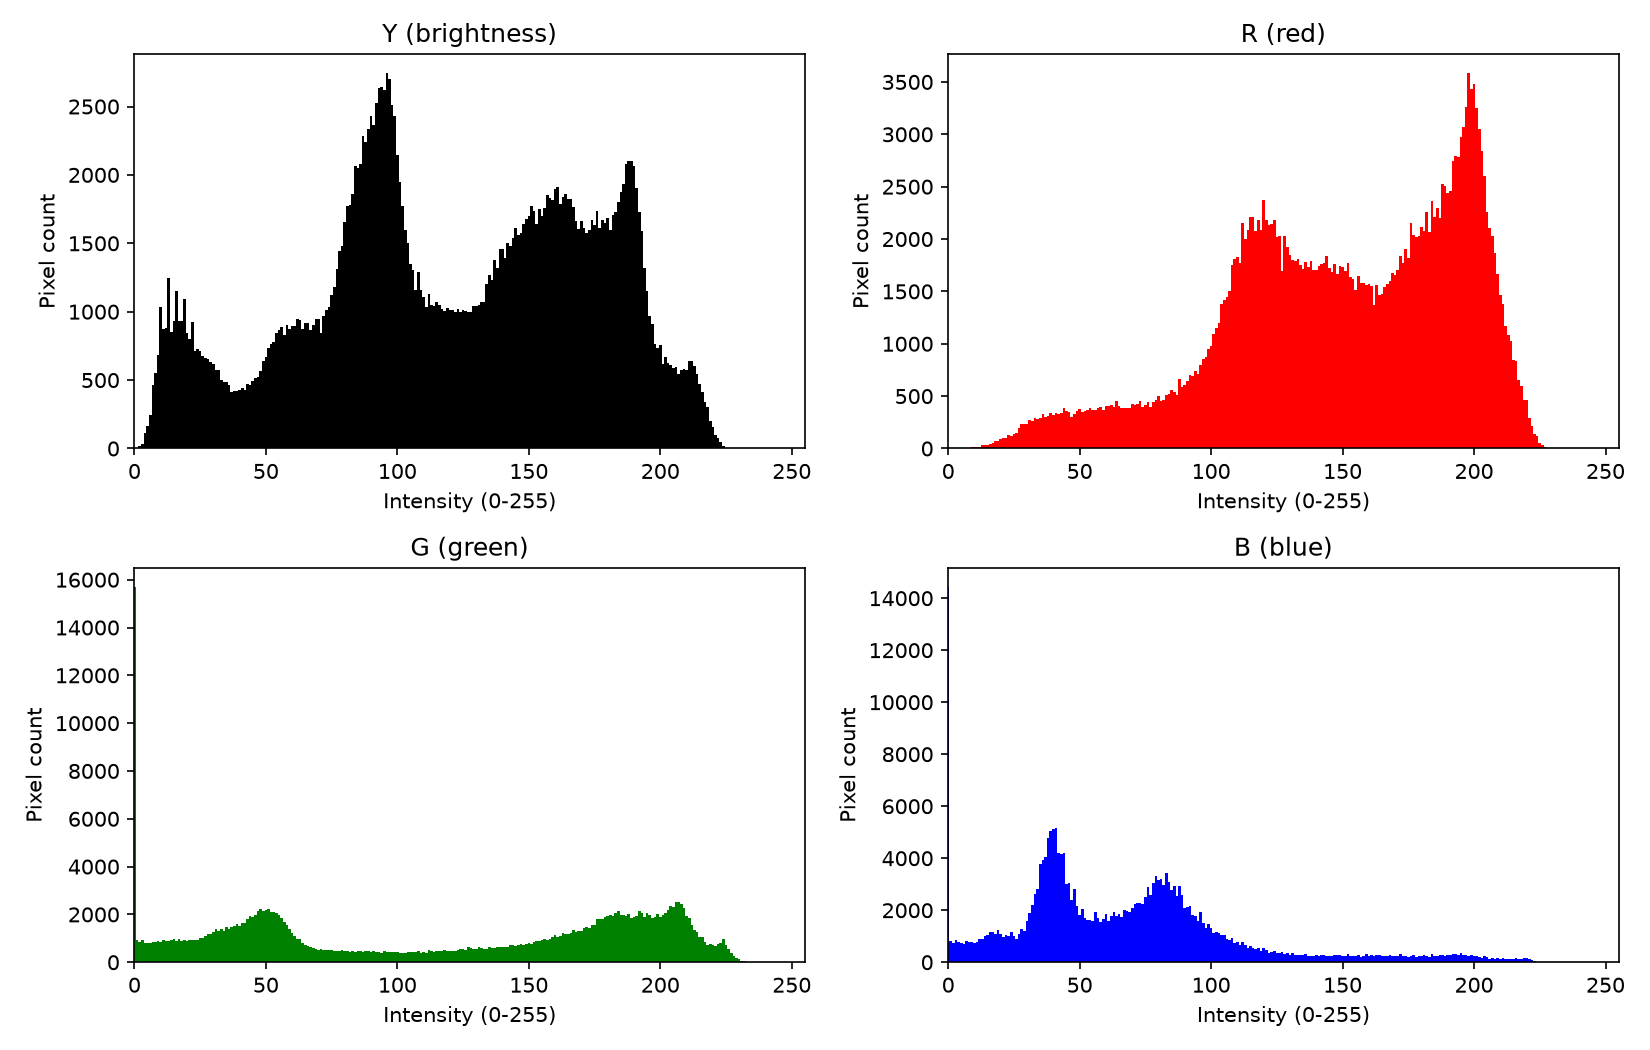
\includegraphics[width=\linewidth]{section2_channel_histograms.png}
\caption{Histograms of the Y (brightness), R, G and B channels used in Q2.1.}
\label{fig:channel-histograms}
\end{figure}

\textbf{Q2.2.} Y was kept and both chroma dimensions were reduced by factors 2, 4 and
8, using area reduction and linear reconstruction. Factor 2 changes \(3N\)
samples to \(N+N/4+N/4=1.5N\): 786,432 to 393,216 bytes, saving 50\%.
Factors 4/8 need 294,912/270,336 bytes, saving 62.5/65.625\%.
These are stored channel samples before display reconstruction, not compressed
files. Factor 2 looked close; factor 4 softened colour boundaries and factor 8
showed clearer blending, while Y detail remained.

\begin{figure}[H]
\centering
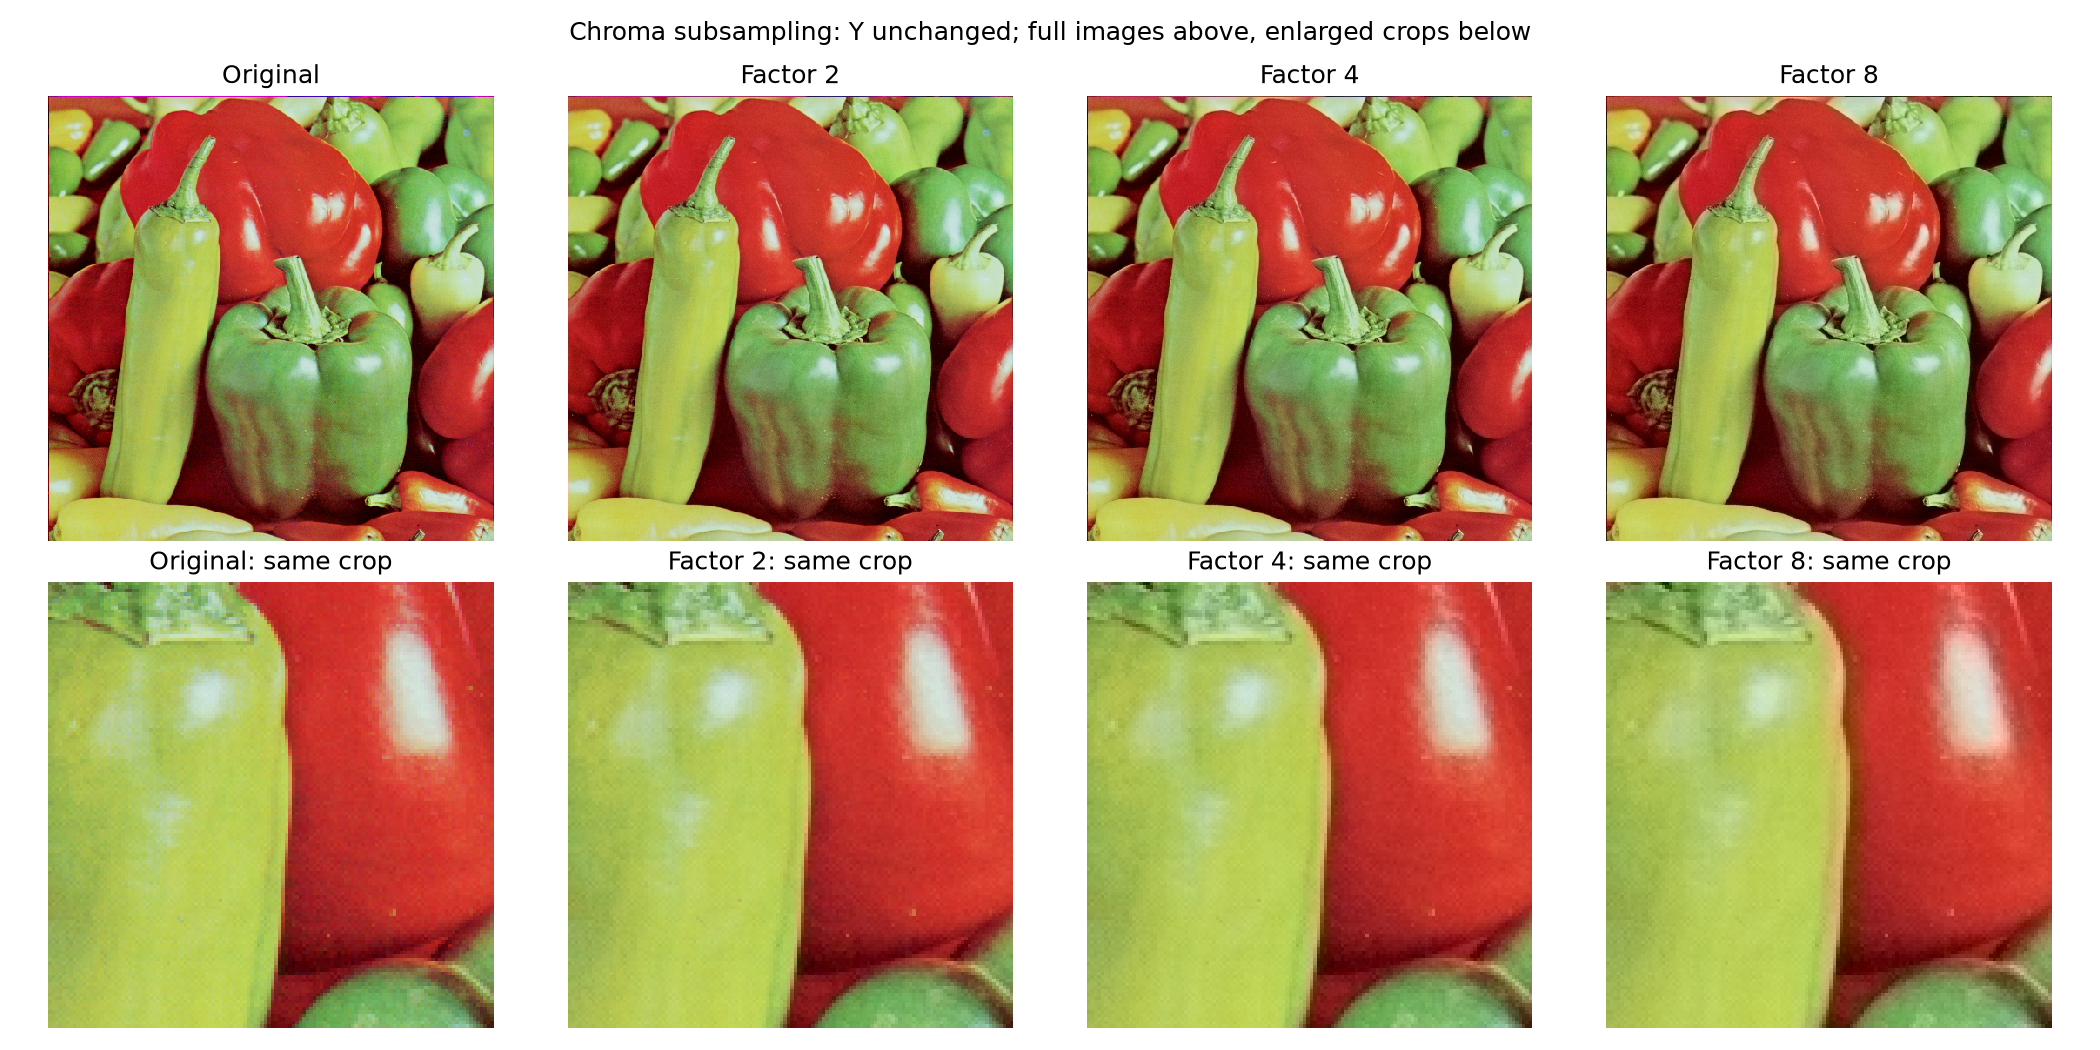
\includegraphics[width=\linewidth]{section2_chroma_subsampling.png}
\caption{Chroma subsampling at factors 2, 4 and 8 compared with the original image. Enlarged crops show increasing colour smoothing while luminance detail is preserved.}
\label{fig:chroma-subsampling}
\end{figure}

\subsection{Quantization and Sampling}
\textbf{Q3.1.} RGB integer division by 16 gave 16 possible levels per channel,
displayed as \(0,16,\ldots,240\). Only 15 were occupied because no input reached
240; smooth colours became slightly stepped and darker. Packed 4-bit storage
would give \(2{:}1\) reduction, or 50\% saving: 393,216 versus 786,432 bytes.
The actual \texttt{uint8} array still occupied 786,432 bytes.

\textbf{Q3.2.} Grayscale division by 32 grouped 32 input intensities into each
of eight levels, displayed as \(0,32,\ldots,224\). All eight were occupied;
the last held only 29 pixels. Both histograms counted 262,144 pixels.
Combining nearby intensities caused banding and lost shading and texture,
although outlines remained clear (Figure~\ref{fig:3bit}).


\begin{figure}[!htbp]
\centering
% Omit only the image row; retain both complete histogram axes.
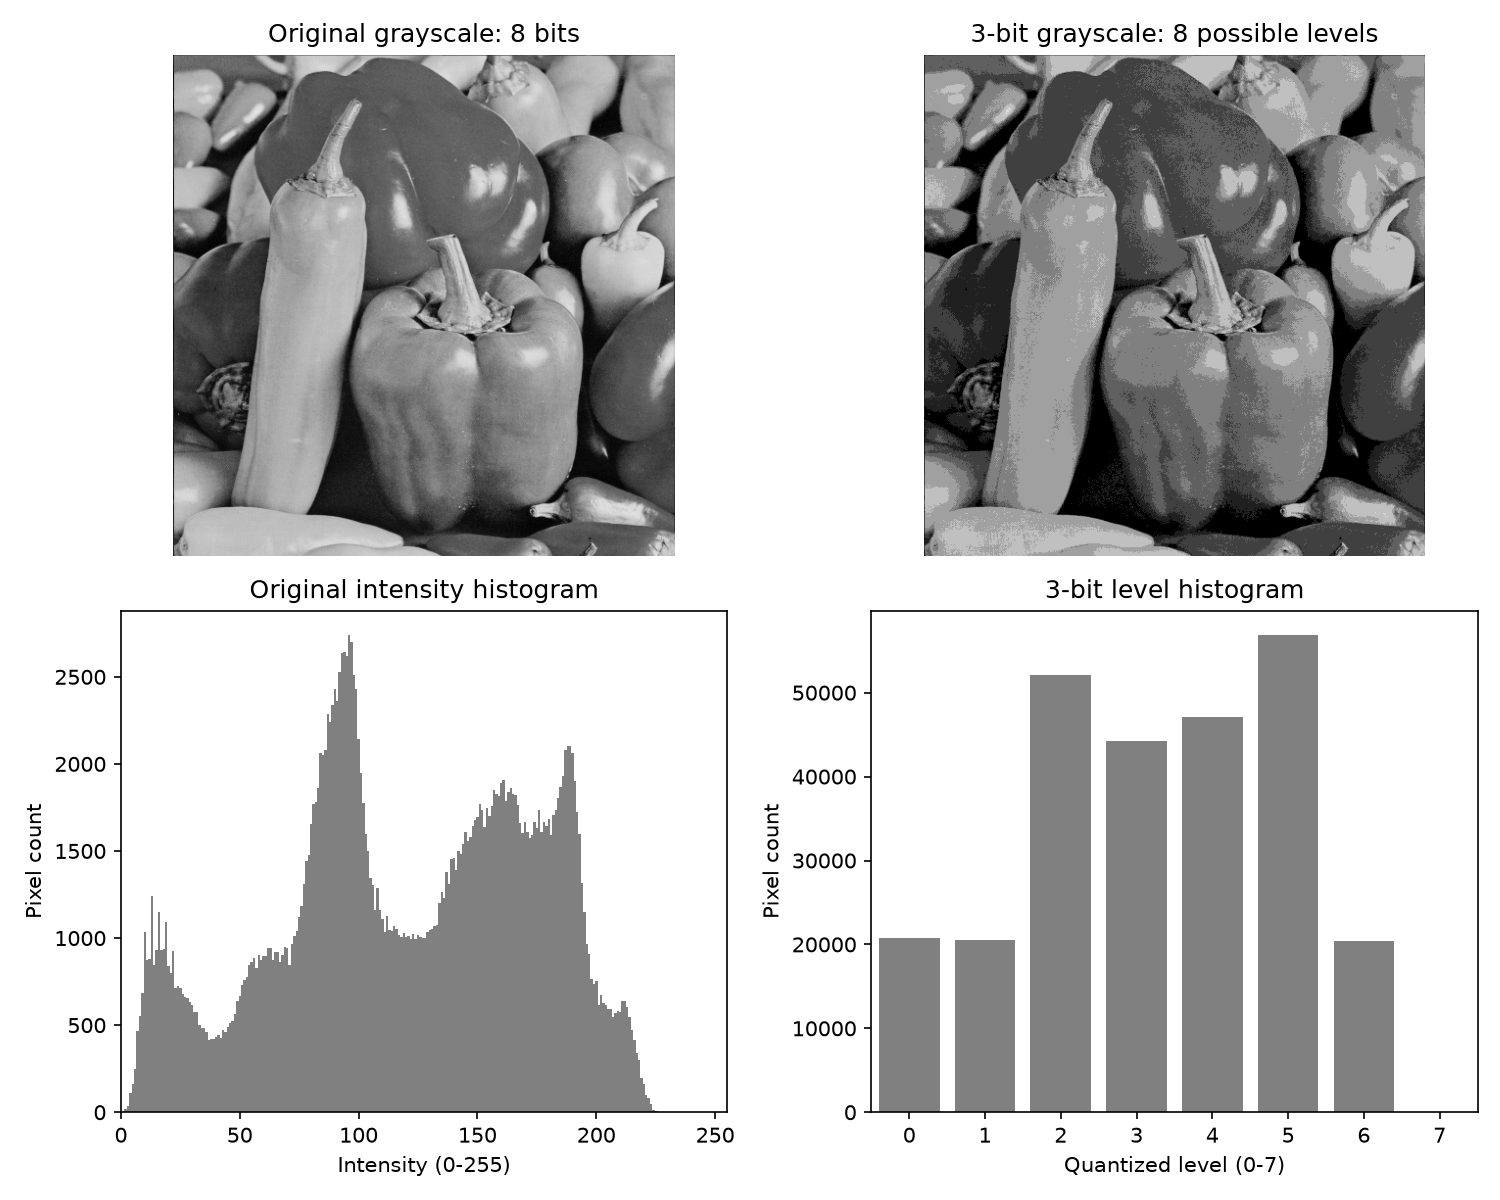
\includegraphics[trim=0 0 0 273.6bp,clip,width=\linewidth]{section3_3bit_histograms.png}
\caption{Q3.2: original intensities (left) and 3-bit levels (right), using separate count scales.}
\label{fig:3bit}
\end{figure}

\subsection{Convolution and Edge Detection}
\textbf{Q4.1.} Matching Gaussian kernels were compared at \(\sigma=1\), using
float64 output and \texttt{BORDER\_REFLECT\_101}, after warm-up
(Table~\ref{tab:times}). Separable filtering was faster only at \(5\times5\);
ordinary 2D was slightly faster at 11 and 21. Costs fall from \(k^2\) to about
\(2k\) weights per pixel, potentially helping large kernels, but library
implementation affects real speed. Both outputs looked alike, differing by
at most about 0.000002 intensity units.

\begin{table}[H]
\centering
\caption{Recorded average times; loading and plotting excluded.}\label{tab:times}
\begin{tabular}{lrrr}\toprule
Task (first / second method) & Runs & First (ms) & Second (ms)\\\midrule
Gaussian \(5\times5\) (2D / separable) & 30 & 5.420 & 1.429\\
Gaussian \(11\times11\) (2D / separable) & 30 & 9.880 & 10.455\\
Gaussian \(21\times21\) (2D / separable) & 30 & 23.481 & 24.022\\
Brightness (NumPy / loops) & 5 & 2.040 & 468.915\\
Log transform (direct / lookup) & 30 & 9.469 & 2.468\\\bottomrule
\end{tabular}
\end{table}

\textbf{Q4.2.} The \(3\times3\) Sobel function used \texttt{dx=0, dy=1}.
Absolute top-to-bottom brightness changes highlighted horizontal boundaries
and weakened long vertical sides. With \texttt{dx=1, dy=0}, vertical edges
stood out; curved edges appeared in both (Figure~\ref{fig:sobel-edges}).

\begin{figure}[H]
\centering
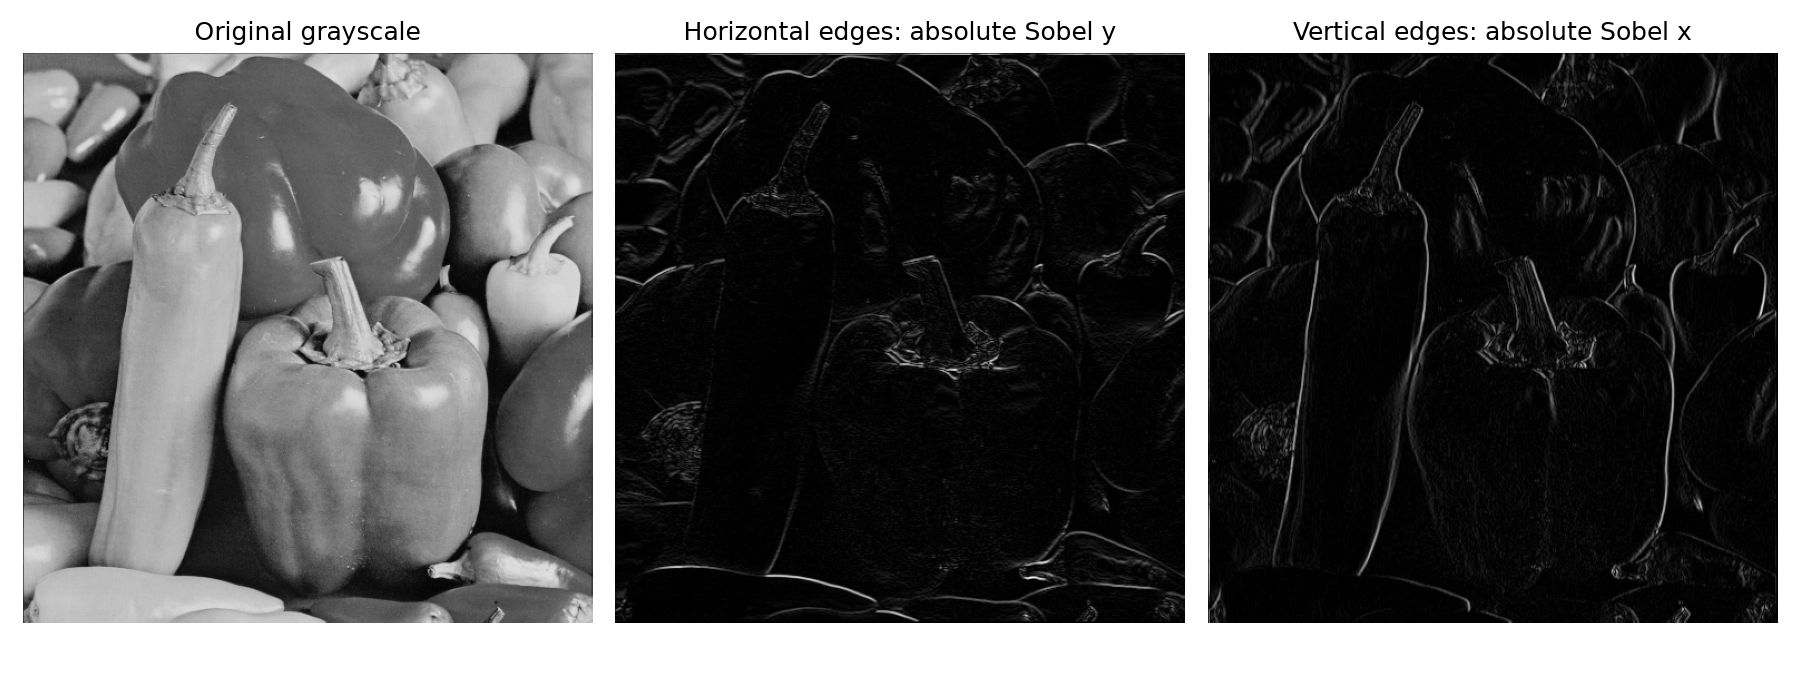
\includegraphics[width=\linewidth]{section4_sobel_edges.png}
\caption{Q4.2: Sobel edge detection. Horizontal edges use \texttt{dy=1}; vertical edges use \texttt{dx=1}.}
\label{fig:sobel-edges}
\end{figure}

\textbf{Q4.3.} Signed derivatives combined as \(G=\sqrt{G_x^2+G_y^2}\);
a copy was normalized to 0--255. Both directions gave more complete outlines
and stems. Brighter pixels mean stronger edges
(Figure~\ref{fig:gradient-magnitude}).

\begin{figure}[H]
\centering
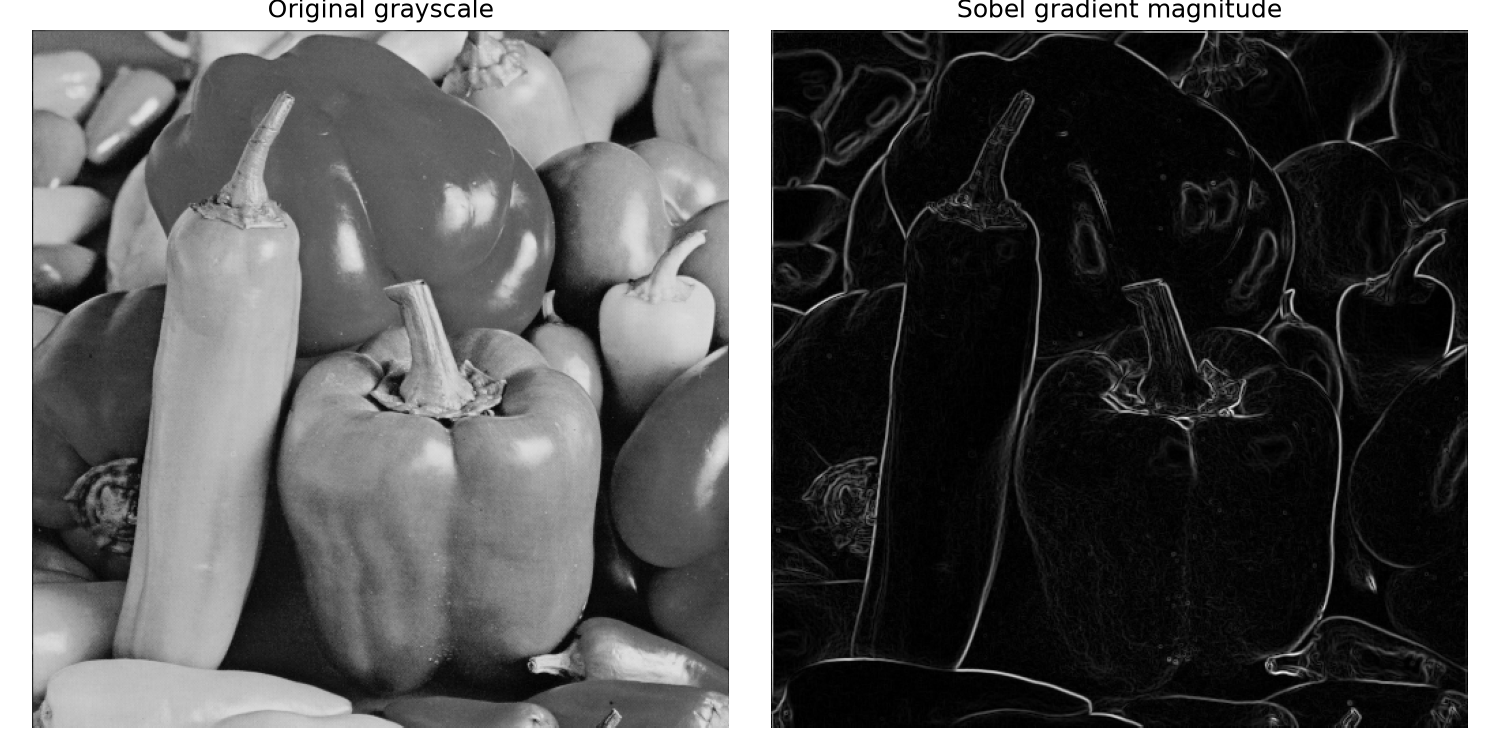
\includegraphics[width=0.85\linewidth]{section4_gradient_magnitude.png}
\caption{Q4.3: Original grayscale image and Sobel gradient magnitude.}
\label{fig:gradient-magnitude}
\end{figure}

\subsection{Matrix Operations}
\textbf{Q5.1.} Stacking pixels, applying \(1.2(I-128)+128+20\), clipping to
0--255 and reshaping gave identical brighter images from NumPy and loops, with
clipped highlights. NumPy was 229.82 times faster from unrounded times
(Table~\ref{tab:times}), avoiding per-pixel Python operations. Timings included
calculation, output creation and conversion.

\textbf{Q5.2.} The stacked image has 262,144 values, so H has
\(262{,}144^2=68{,}719{,}476{,}736\) elements. Float32 needs
274,877,906,944 bytes (256 GiB); float64 needs 549,755,813,888 bytes (512 GiB),
where GiB is \(1024^3\) bytes. H was not allocated. Most entries would be zero;
keeping nine kernel weights and processing local neighbourhoods is more practical.

\subsection{Pixel-Based Processing}
\textbf{Q6.1.} Direct and 256-entry lookup versions gave identical
\texttt{uint8} images, range 0--240. Lookup was 3.84 times faster
(Table~\ref{tab:times}) because it reused results instead of recalculating
logarithms. Its separate 0.539 ms construction was excluded; applications
were warmed up and averaged over 30 calls.

\textbf{Q6.2.} Two log halves joined at 127.5, strength 4
(Figure~\ref{fig:gamma-log}, right). The curve is steeper centrally and flatter
at both ends: input gaps of 32 gave output gaps 17 (0--32), 64 (112--144), and
18 (223--255). Middle shading separated more; shadow/highlight differences
compressed. Dark gaps looked darker and light areas brighter. Intensity order
and endpoints 0 and 255 were preserved.


\begin{figure}[!htbp]
\centering
\begin{minipage}[b]{0.49\linewidth}\centering
% Right histogram only, with its title, axes and all tick labels.
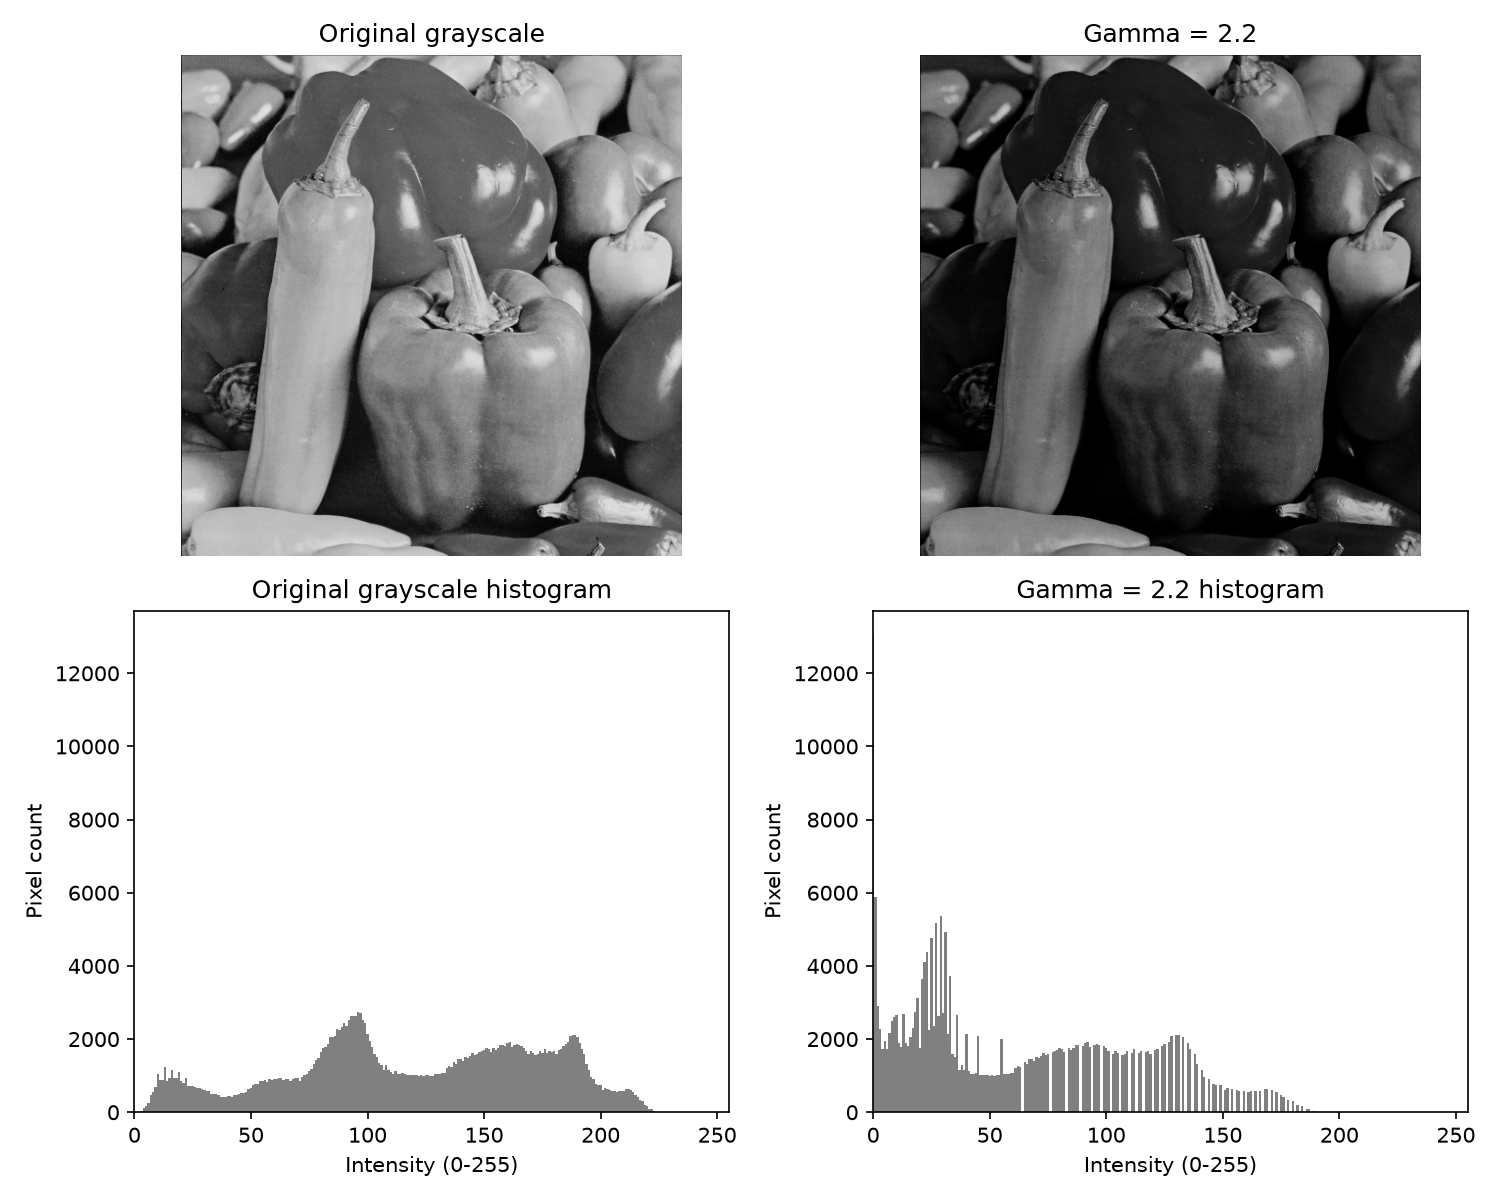
\includegraphics[trim=360bp 0 0 273.6bp,clip,width=\linewidth]{section1_gamma_histograms.png}
\end{minipage}\hfill
\begin{minipage}[b]{0.49\linewidth}\centering
% Retain the complete transfer-function panel and its legend.
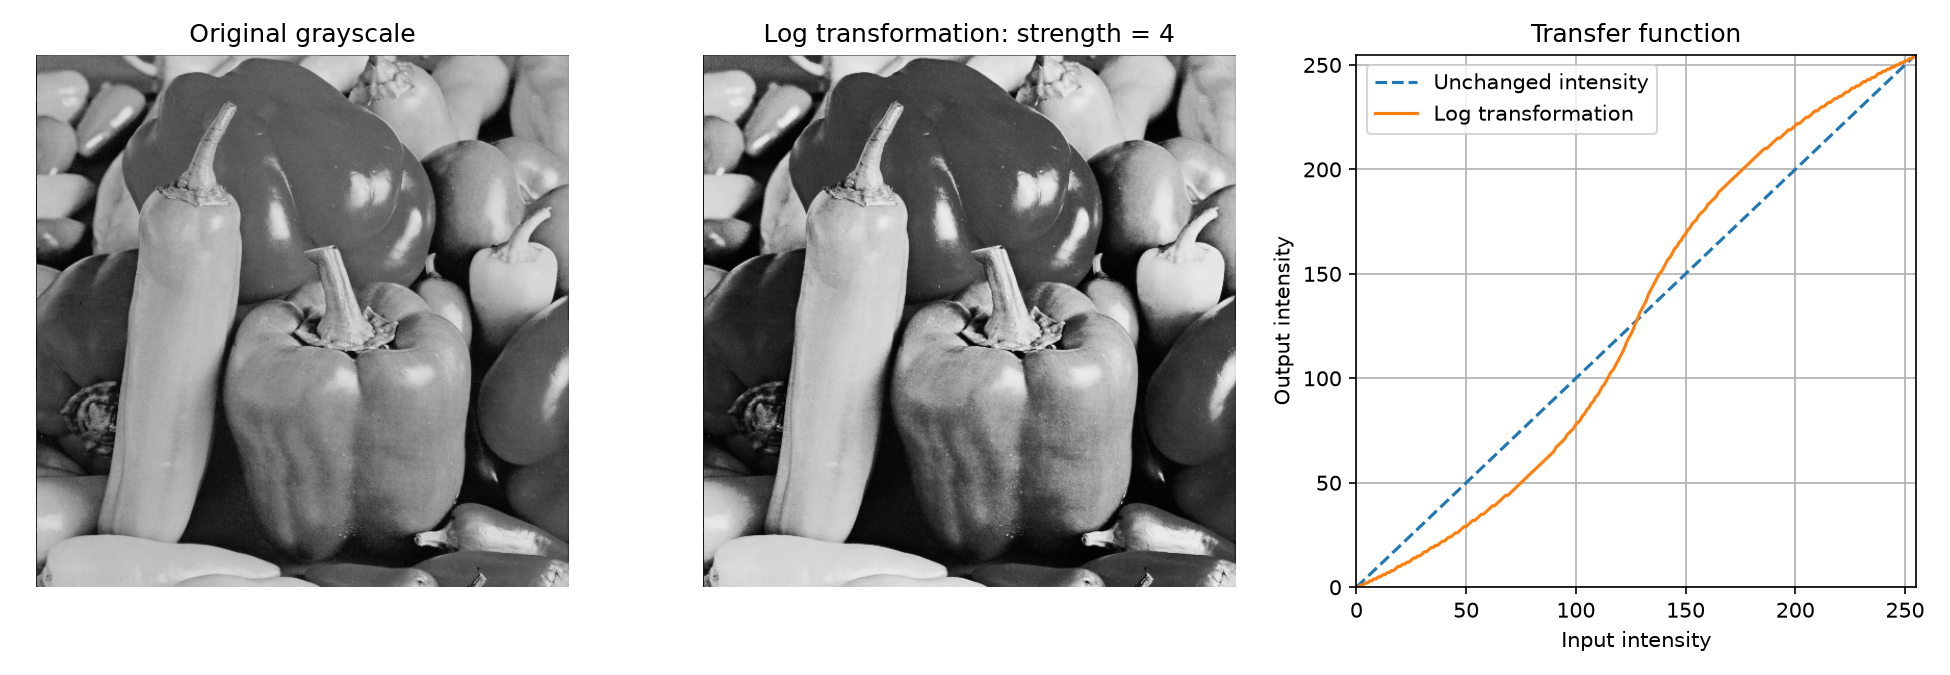
\includegraphics[trim=609.6bp 0 0 0,clip,width=\linewidth]{section6_log_transformation.png}
\end{minipage}
\caption{Left: gamma-2.2 histogram, compared with Figure~\ref{fig:3bit}'s original
using its labelled count scale. Right: Q6.2 logarithmic transfer function;
the dashed line leaves intensity unchanged.}
\label{fig:gamma-log}
\end{figure}

\subsection{Elementary Images}
\textbf{Q7.1.} Outer products of the teacher's vectors made \(16\times16\)
images. Ramp\(\times\)Ramp gave smooth two-direction changes;
Step\(\times\)Ramp a boundary plus a gradient; Step\(\times\)Step a sharp
lower-right block; Step\(\times\)Sine repeating columns in the lower half.
The shared \(-1\) to 1 scale made zero middle gray. See Figure~\ref{fig:elementary-images}.

\begin{figure}[!htbp]
\centering
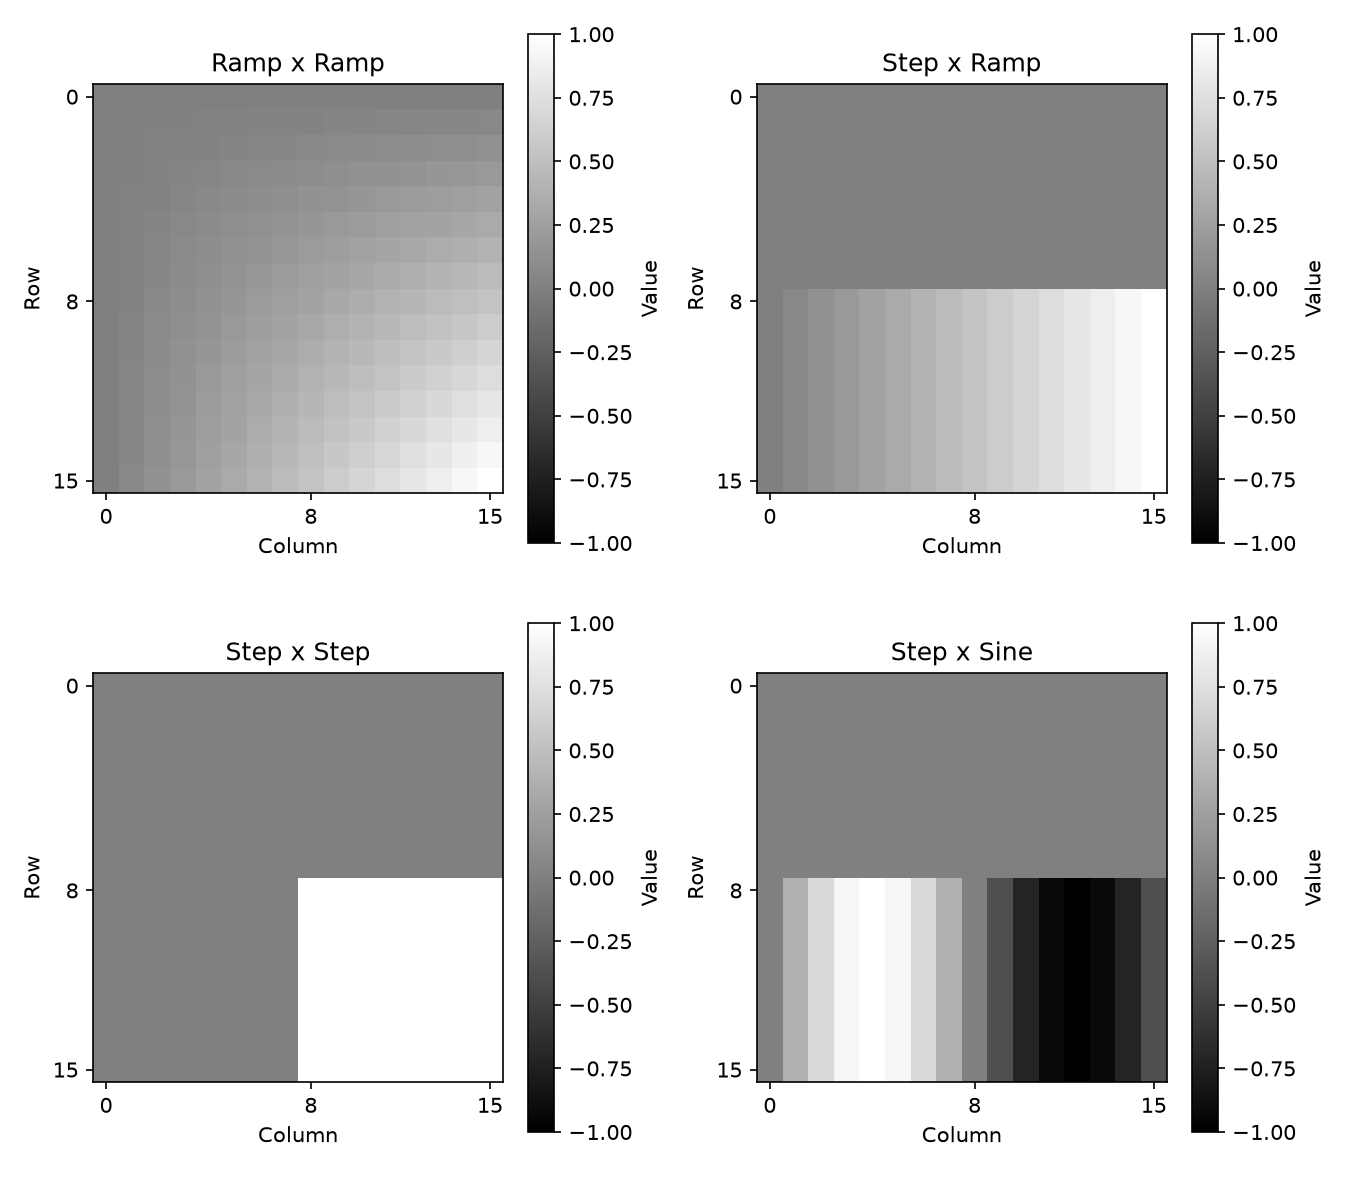
\includegraphics[width=0.85\linewidth]{section7_elementary_images.png}
\caption{Q7.1: Four elementary \(16\times16\) images generated from combinations of ramp, step and sine basis vectors.}
\label{fig:elementary-images}
\end{figure}

\begin{samepage}
\textbf{Q7.2.} Least squares fitted Step\(\times\)Ramp, Step\(\times\)Step and
Step\(\times\)Sine to the \(8\times8\) square (rows 8--15, columns 4--11,
zero-based). Weights were 0.156058, 0.812731 and 0.688038;
MSE 0.107400 on 0--1, raw range 0.000000--0.895961. The horizontal boundary
matched, but interiors were uneven, side edges wrong and bands remained
outside the square. Three patterns gave a coarse fit.
\par\end{samepage}


\subsection{Transforms and Frequency Domain}
\textbf{Q8.1.} The display used \texttt{log1p(abs(fftshift(fft2(gray))))}.
The bright centre held average brightness and slow changes; faster changes
lay farther out. Horizontal/vertical streaks included edges and border effects:
vertical edges contribute along horizontal frequency and vice versa.
Curves involve several directions. The FFT does not locate individual edges. See Figure~\ref{fig:fft-spectrum}.

\begin{figure}[!htbp]
\centering
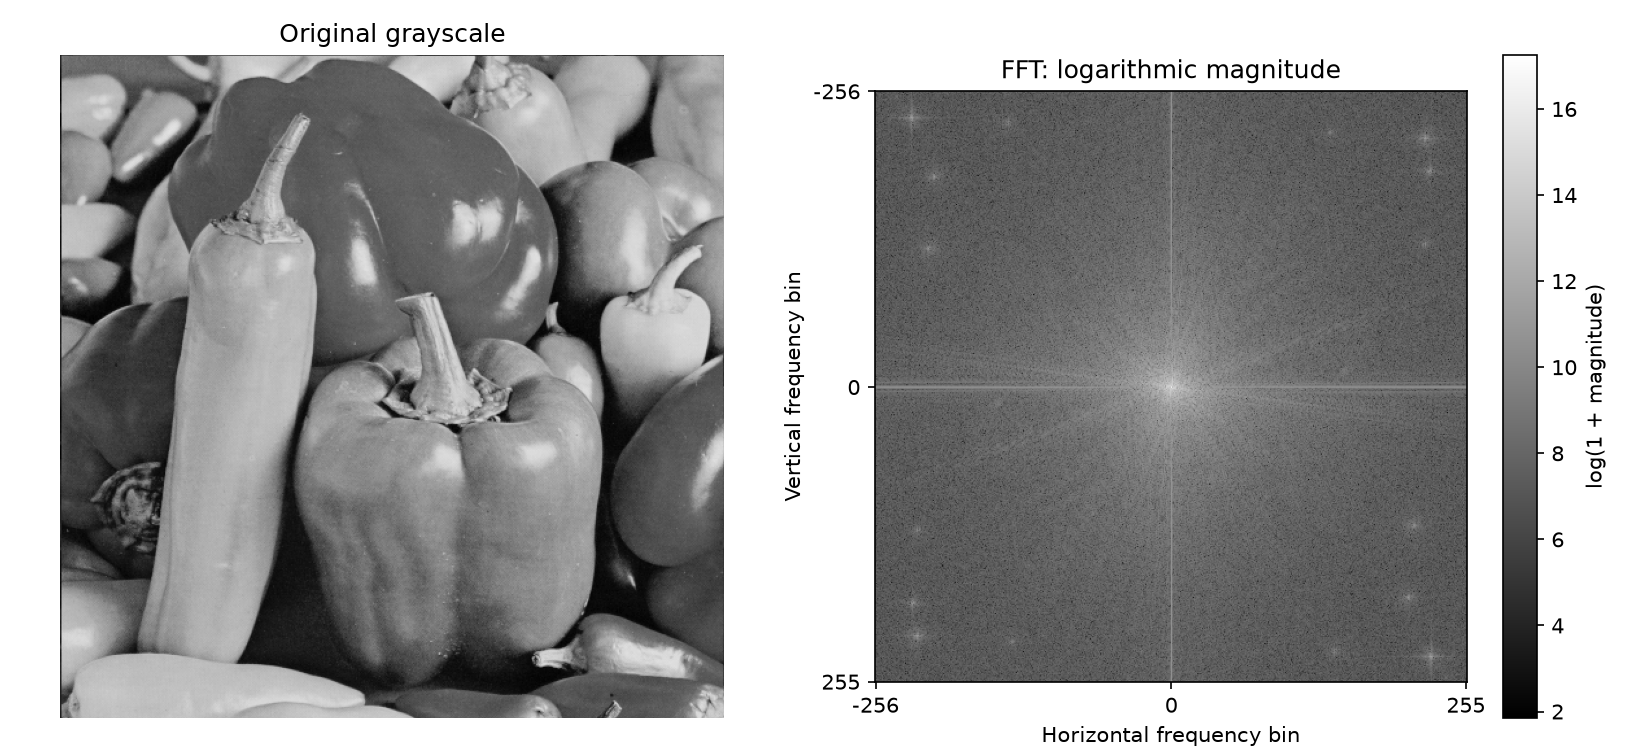
\includegraphics[width=0.85\linewidth]{section8_fft_spectrum.png}
\caption{Q8.1: Original grayscale image and its centered 2D FFT magnitude spectrum (log scale).}
\label{fig:fft-spectrum}
\end{figure}

\textbf{Q8.2.} A circular low-pass mask kept radii below 40 bins in the
\(512\times512\) grid; inverse shifting and FFT returned its real part.
Main shapes remained, detail weakened and boundaries softened, with ringing
from the sharp cutoff. Raw values were
\(-17.078\) to 243.781; negatives displayed black without changing the data.

\textbf{Q8.3.} Floating-point original-minus-low-pass kept outlines, stems and
detail around near-zero smooth regions. The raw range was \(-155.400\) to
113.396; display limits were \(\pm155.400\), with zero middle gray.
Ringing remained. Low-pass plus high-pass recovered the original with maximum
error 0; the inverse FFT's largest imaginary part was \(6.172\times10^{-14}\). See Figure~\ref{fig:frequency-filtering}.


\begin{figure}[!htbp]
\centering
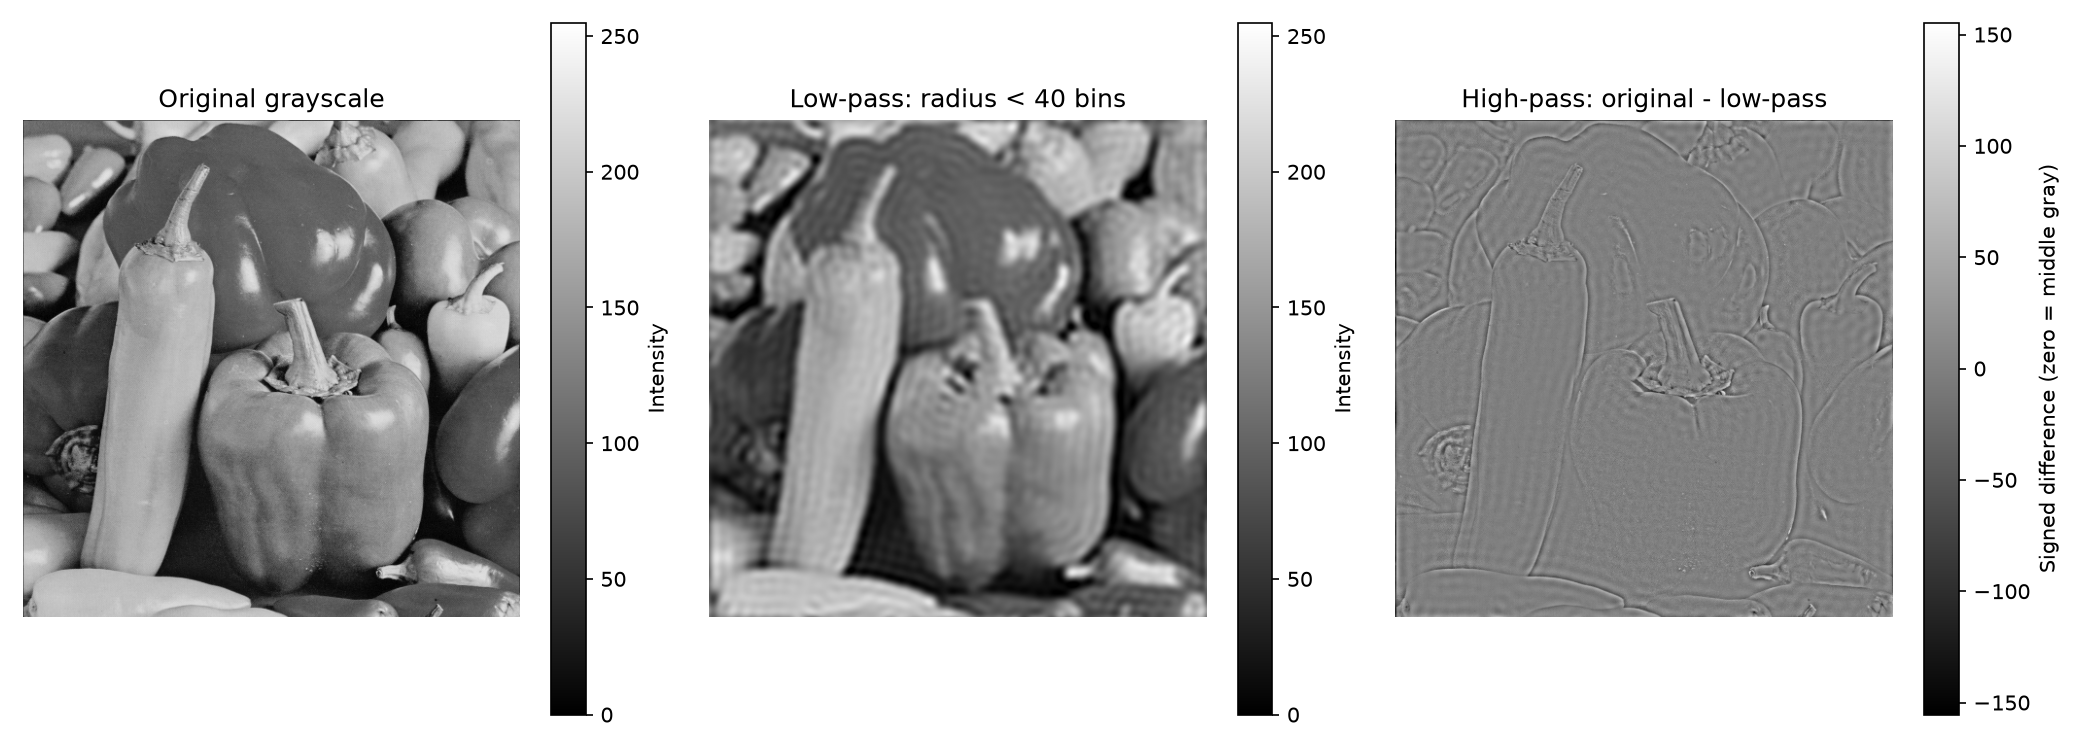
\includegraphics[width=\linewidth]{section8_frequency_filtering.png}
\caption{Q8.2--8.3: Original grayscale image, low-pass result (radius below 40 bins), and signed high-pass difference. Zero is middle gray in the high-pass image.}
\label{fig:frequency-filtering}
\end{figure}

\subsection{Histograms and Image Enhancement}
\textbf{Q9.1.} Figure~\ref{fig:hist} shows that pixel
intensities are concentrated mainly in the darker and
middle ranges. The largest histogram peak was at
intensity 96, and 76.43\% of pixels were between 64
and 191. This indicates that the image contains mostly
midtones and darker areas, with relatively few bright
pixels. The cumulative histogram confirms this:
52.51\% of pixels had intensities at or below 127,
and 92.19\% were at or below 191. It reached 100\%
at intensity 228. The histograms describe how
brightness is distributed, but not where individual
objects or details appear in the image.

\begin{figure}[!htbp]
\centering
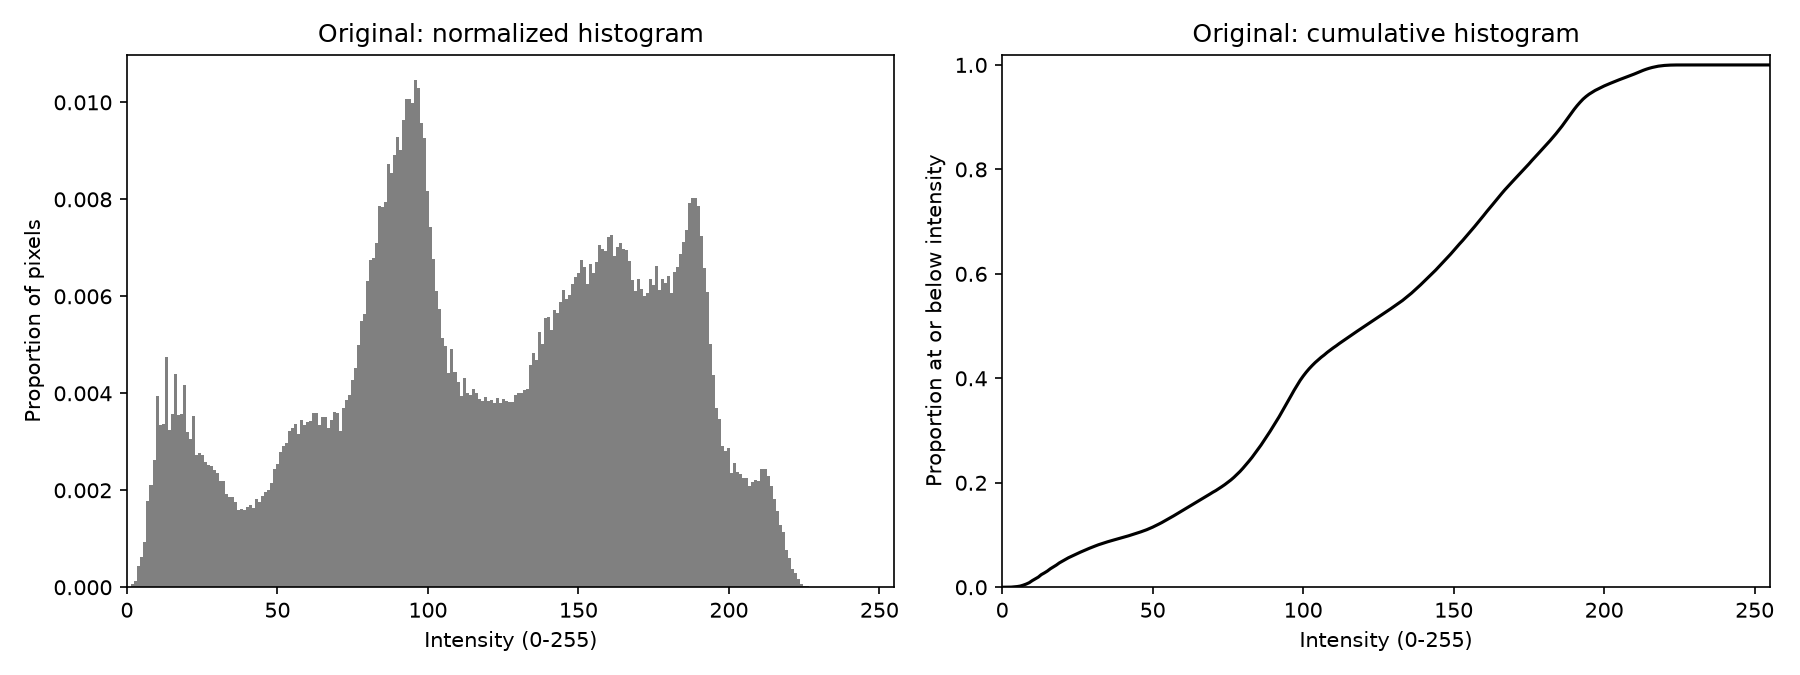
\includegraphics[width=\linewidth]{section9_histograms.png}
\caption{Q9.1: original normalized histogram and cumulative histogram (CDF).}
\label{fig:hist}
\end{figure}

\begin{samepage}
\textbf{Q9.2.} Reducing contrast with
\(128+0.5(I-128)\) compressed the grayscale range
from 0--228 to 64--178, making the image flatter
and reducing differences between dark and light
regions. Histogram equalization using
\(T(r)=255\,\mathrm{CDF}(r)\) expanded the intensity
range to 0--255. Compared with the reduced-contrast
image, shading and details became clearer. Compared
with the original, dark and light regions showed
stronger contrast, although grain became more visible
(Figure~\ref{fig:equalization}). The custom CDF
method and OpenCV's \texttt{equalizeHist()} produced
nearly identical results, with a maximum difference
of 1 intensity level and a mean absolute difference
of 0.443756. The small differences arise from
OpenCV's cumulative-histogram normalization and
rounding, compared with the simpler implemented
transformation.
\par\end{samepage}



\begin{figure}[!htbp]
\centering
\begin{minipage}[b]{0.185\linewidth}\centering Original\\[2pt]
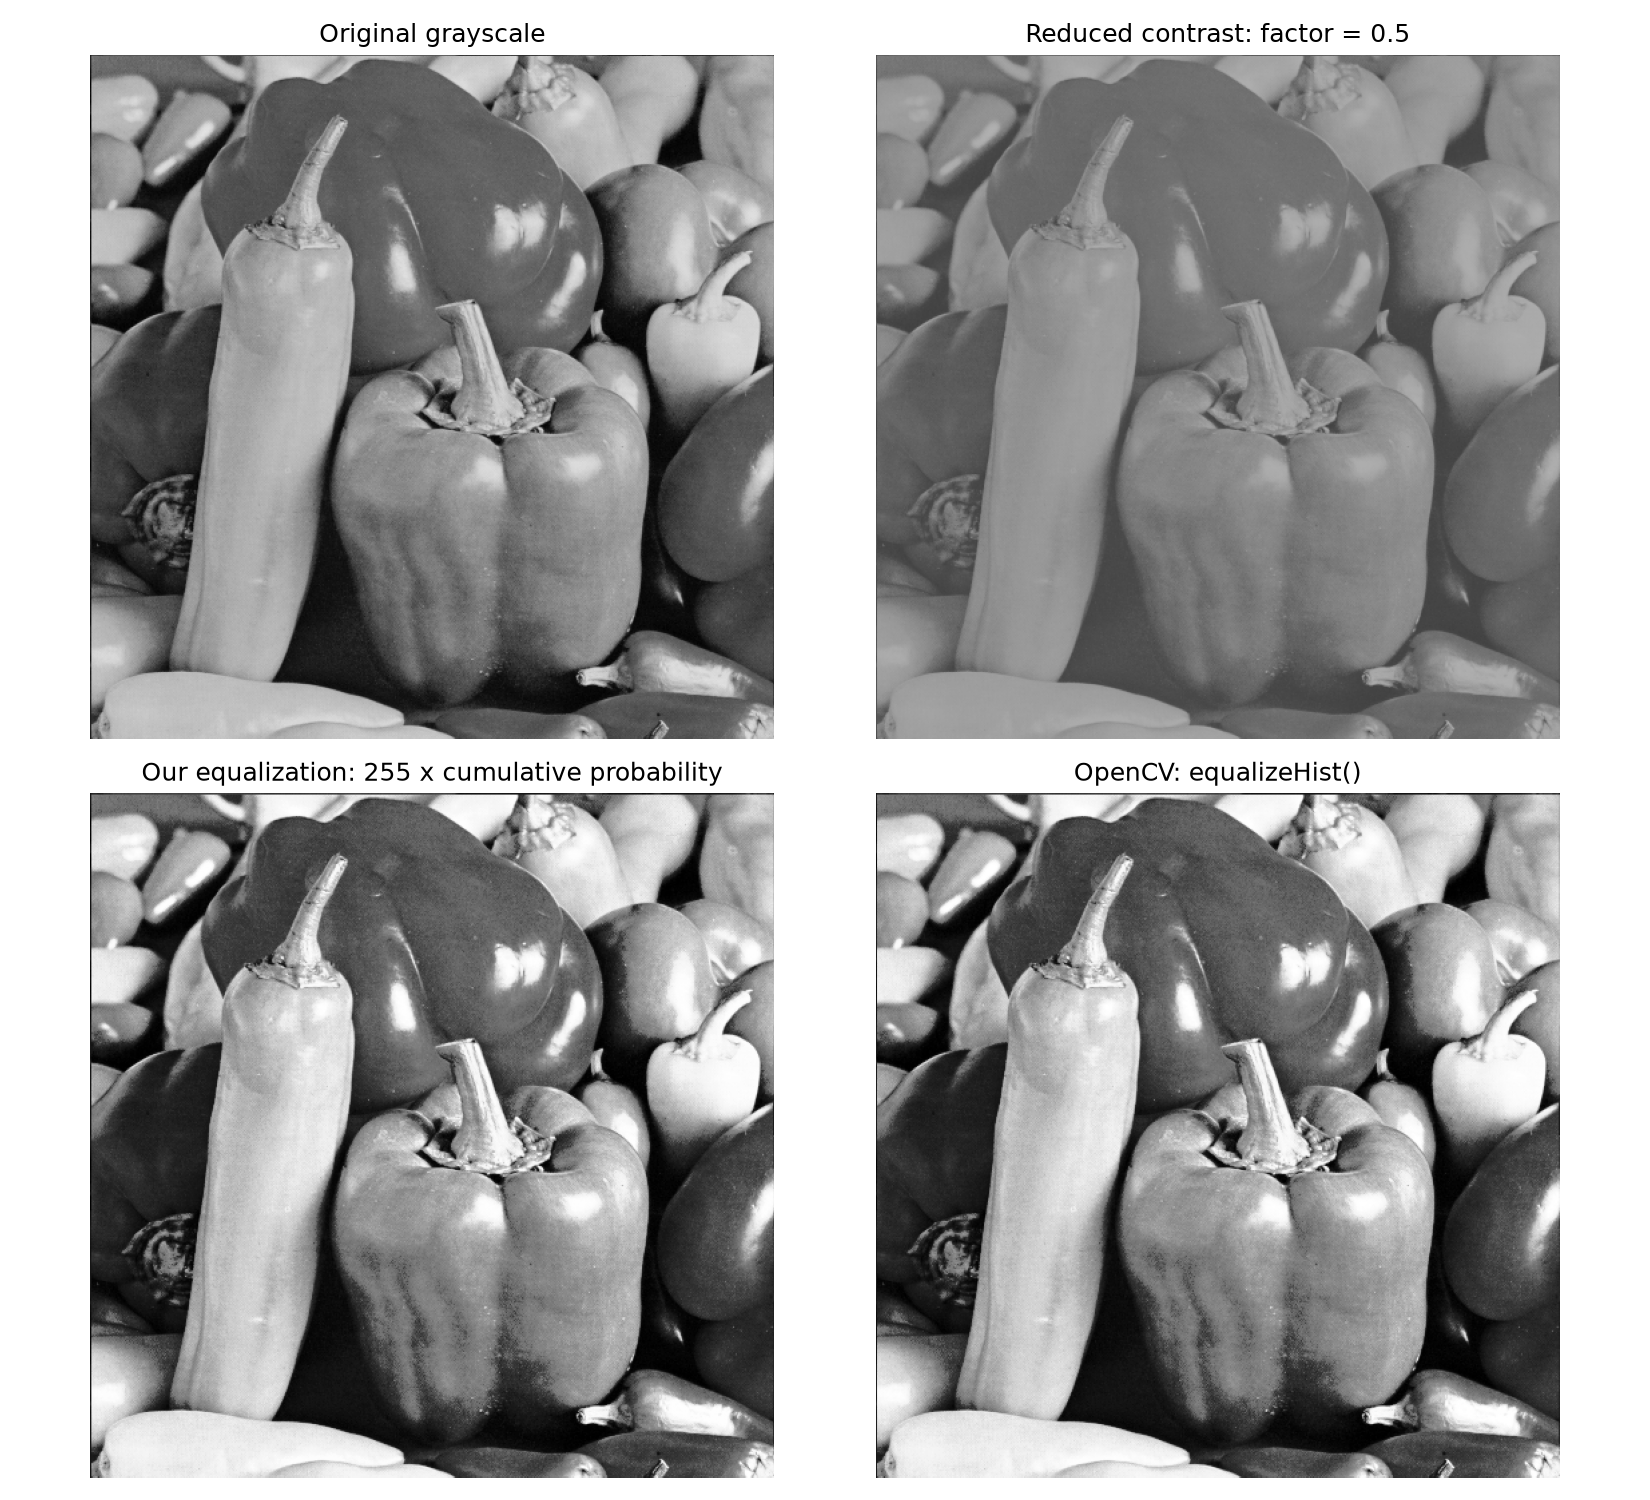
\includegraphics[trim=43.2bp 365.28bp 420.48bp 26.4bp,clip,width=\linewidth]{section9_histogram_equalization.png}
\end{minipage}\hfill
\begin{minipage}[b]{0.185\linewidth}\centering Contrast 0.5\\[2pt]
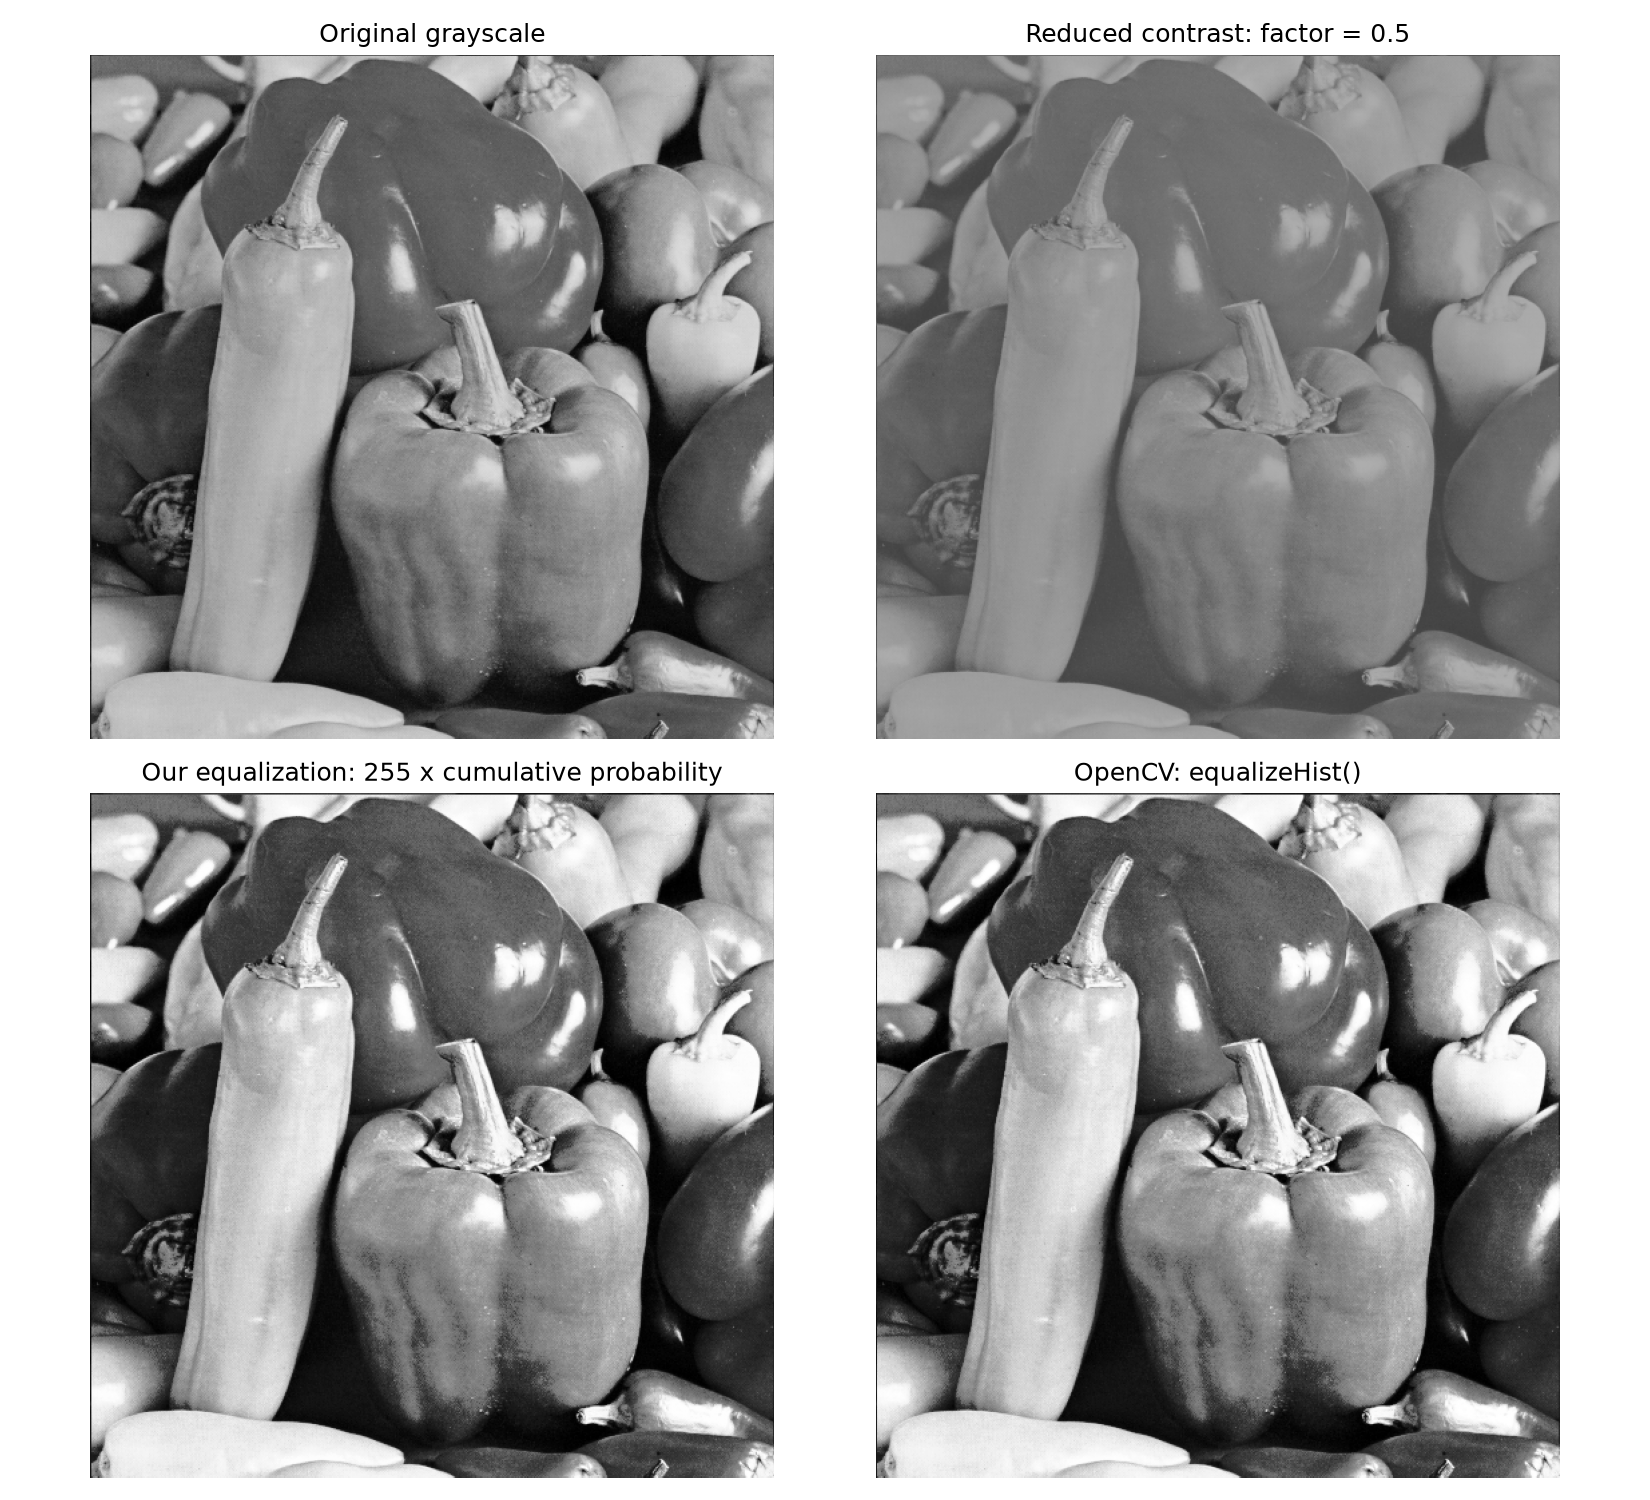
\includegraphics[trim=420.48bp 365.28bp 43.2bp 26.4bp,clip,width=\linewidth]{section9_histogram_equalization.png}
\end{minipage}\hfill
\begin{minipage}[b]{0.185\linewidth}\centering CDF method\\[2pt]
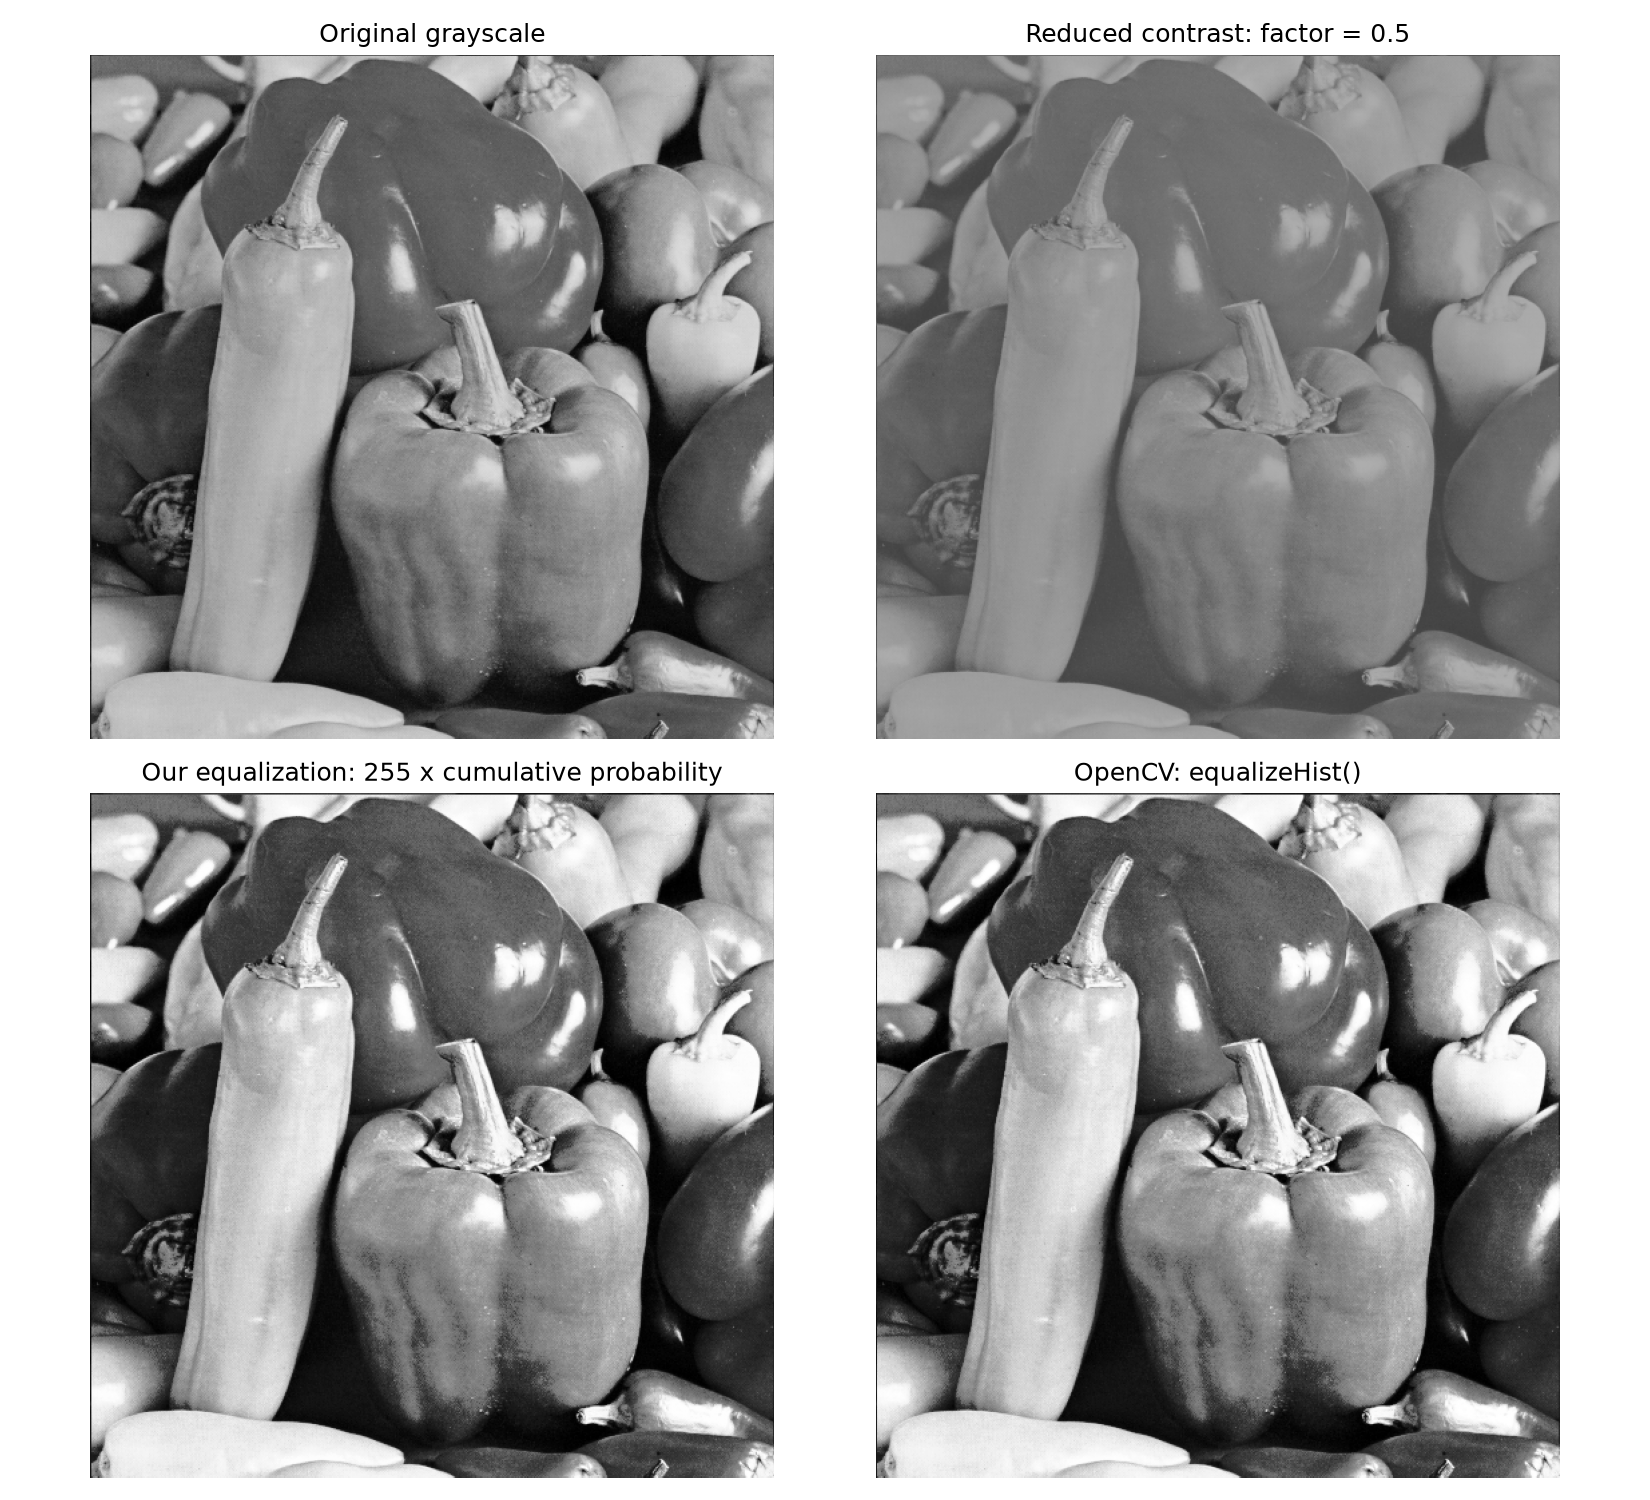
\includegraphics[trim=43.2bp 10.56bp 420.48bp 381.12bp,clip,width=\linewidth]{section9_histogram_equalization.png}
\end{minipage}\hfill
\begin{minipage}[b]{0.185\linewidth}\centering OpenCV\\[2pt]
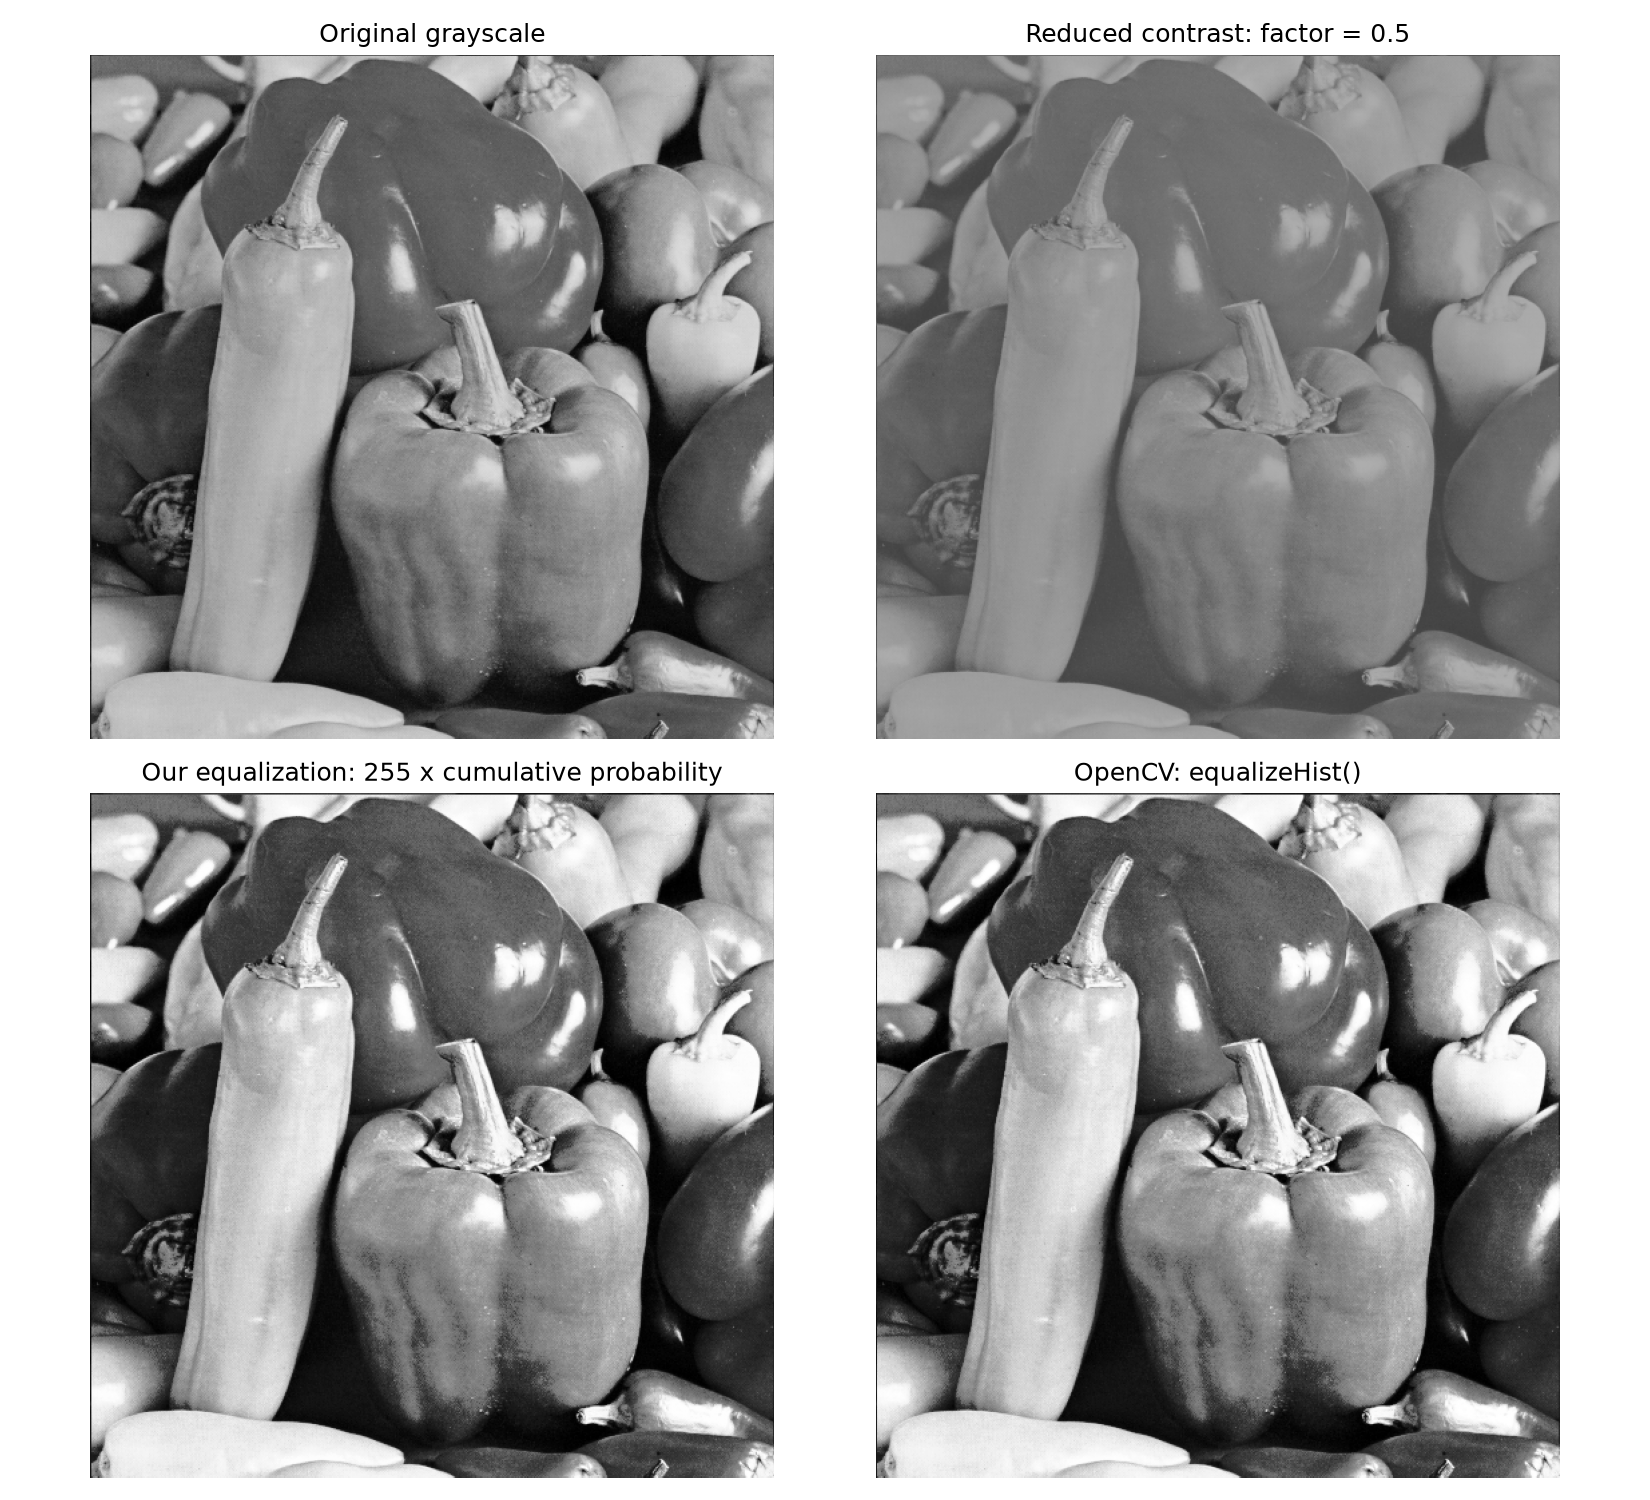
\includegraphics[trim=420.48bp 10.56bp 43.2bp 381.12bp,clip,width=\linewidth]{section9_histogram_equalization.png}
\end{minipage}\hfill
\begin{minipage}[b]{0.185\linewidth}\centering Sobel\\[2pt]
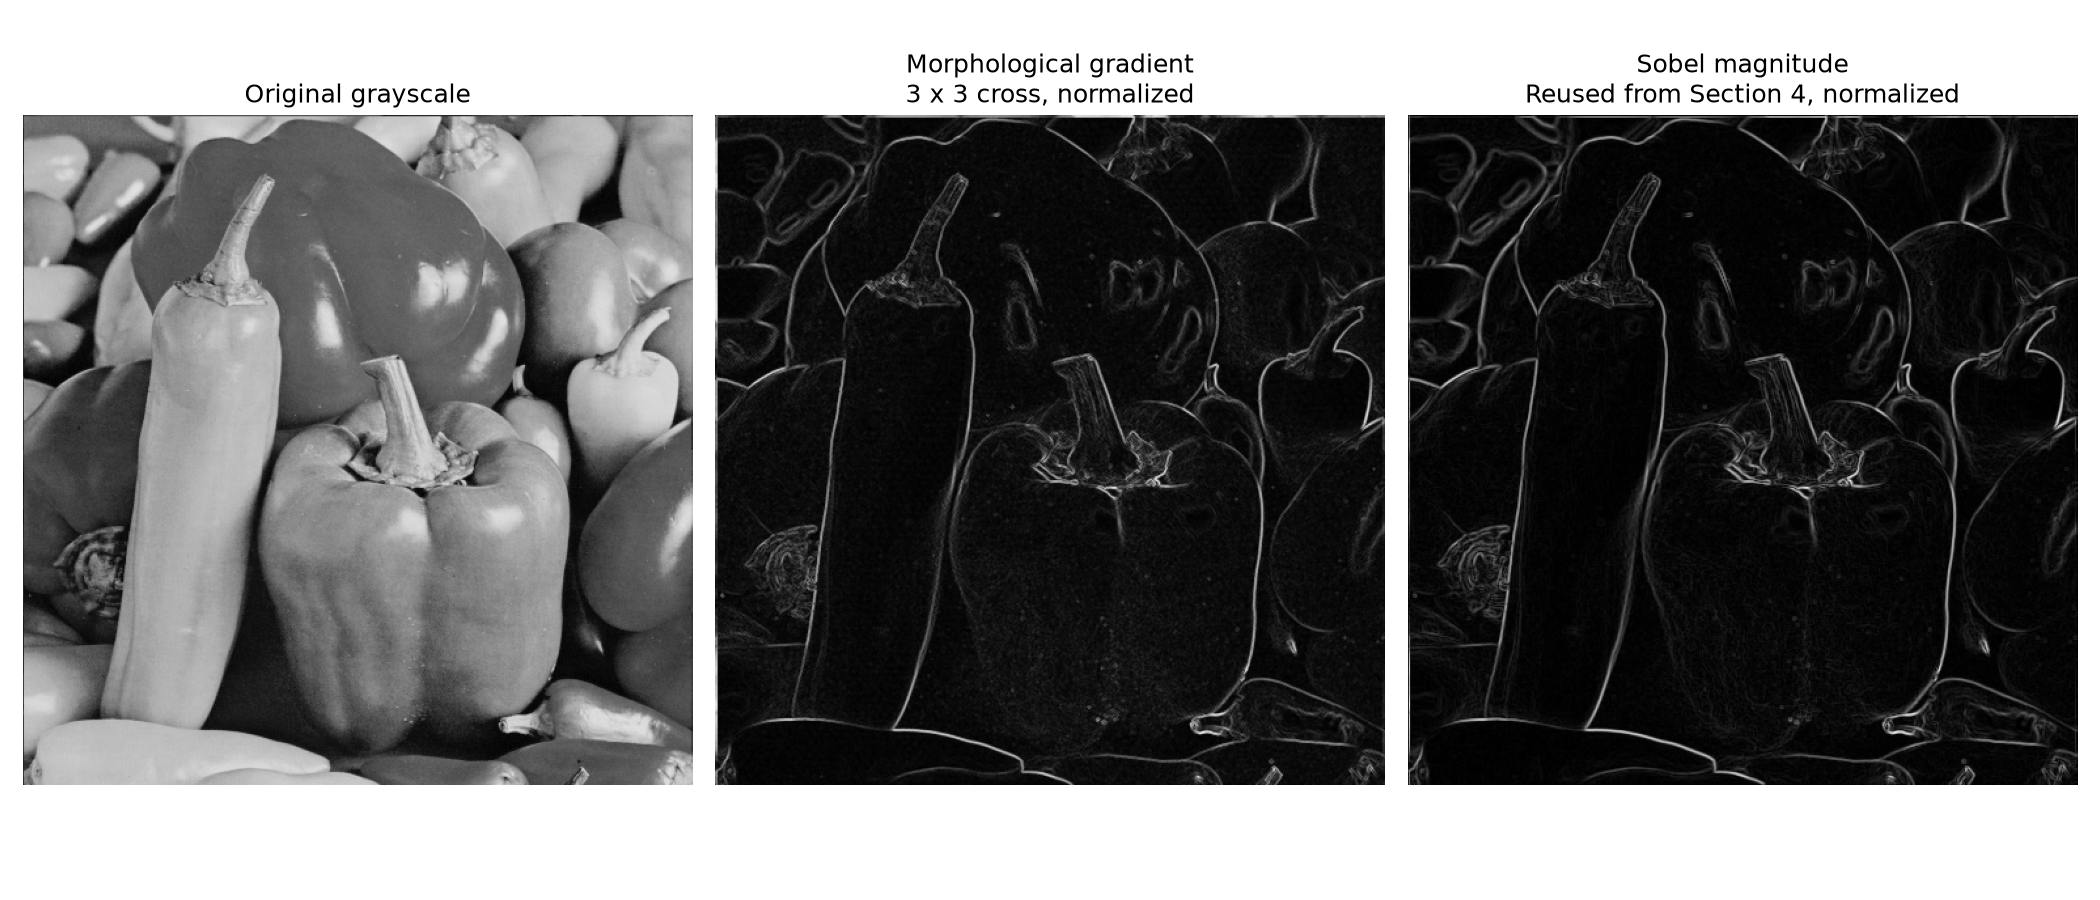
\includegraphics[trim=675.84bp 55.2bp 10.56bp 55.2bp,clip,width=\linewidth]{section11_gradient_comparison.png}
\end{minipage}
\caption{Q9.2: contrast/equalization (left four); Q4.3: normalized Sobel (right). Displays: 0--255.}
\label{fig:equalization}
\end{figure}

\subsection{Noise and Noise Reduction}
\textbf{Q10.1.} With seed 42, one zero-mean Gaussian sample was scaled and added
in floating point, then clipped before integer conversion. Median \(3\times3\)
at noise \(\sigma=25\) changed PSNR from 20.318 to 26.829 dB; bilateral
(diameter 9, colour/spatial sigmas 75/75) at \(\sigma=35\) changed 17.519 to
26.888 dB. The 0.059 dB gap closely matched outputs, but different input noise
prevents a same-input ranking. Bilateral trials at \(\sigma=25,30,35\) gave
28.860, 28.004, 26.888 dB. Both reduced grain; bilateral looked smoother but
softened stems. Similar PSNR did not mean identical appearance.

\textbf{Q10.2.} Both \(3\times3\) filters received the same noisy image for each
row of Table~\ref{tab:noise}. Salt-and-pepper probability was 4\% total
(2\% black, 2\% white without overlap); 3.986\% of pixels were selected.
Mean filtering gave slightly better Gaussian results but blurred edges.
Median removed isolated extremes much better; mean filtering spread them
into gray marks. \texttt{cv2.PSNR()} used the clean image, with differences from unrounded values.

\begin{table}[H]
\centering
\caption{Same-input filtering: PSNR and mean-minus-median difference, all in dB.}
\label{tab:noise}
\begin{tabular}{lrrrr}\toprule
Noise & Input & Mean & Median & Difference\\\midrule
Gaussian, \(\sigma=25\) & 20.318 & 27.237 & 26.829 & \(+0.409\)\\
Salt-and-pepper, 4\% & 19.296 & 26.516 & 34.035 & \(-7.519\)\\\bottomrule
\end{tabular}
\end{table}

\subsection{Morphological Filtering}
\textbf{Q11.1.} Two \(128\times128\) binary tests used separate shapes.
A had a circle, rectangle and triangle; B added a second circle of a different
size. Each had three white specks and a \(2\times2\) black hole. Opening with a
\(3\times3\) cross removed specks; closing with a \(5\times5\) ellipse filled
the hole. Eight-connected labels minus background gave expected/detected counts
3/3 and 4/4. Corners rounded slightly; touching objects would count together.

\textbf{Q11.2.} Dilation minus erosion with the cross showed pepper boundaries
and more grain; Sobel outlines were smoother. Raw ranges were 0--204 and
0--812.857, separately normalized to 0--255 for display, so displayed brightness
does not compare raw strength. Morphology suits binary shapes and kernel-dependent
boundaries; Sobel suits grayscale brightness changes and directional derivatives.
Its magnitude shows strength, not direction.

\section{Discussion}
Vectorization and lookup saved time with identical outputs. Gaussian timings
depended on routines, not just operation counts; one run cannot give a general
ranking. Filters traded noise against detail and depended on noise type.
Equalization also exposed grain. The coarse shape fit and touching-object limit
show why settings and representation matter.

\section{Conclusion}
The experiments linked pixel values, colour, detail and frequency content.
Numerical results supported the image comparisons and explained time, memory
and noise trade-offs.

\section*{Appendix: Code Snippets}
\textbf{FFT filtering.} The circular mask keeps low frequencies; the inverse FFT returns the smooth image.
\lstinputlisting[firstline=512,lastline=513]{../lab3.py}

\end{document}
